\documentclass{szzclass}
\usepackage{dependencies/szz-math}
\usepackage[czech]{babel}

\subject{BEZ}
\code{BI-SPOL-7}
\topic{Symetrické šifry blokové a proudové (AES, 3DES, RC4) základní parametry, operační módy blokových šifer (ECB, CBC, CFB, OFB, CTR, MAC), jejich základní popis a slabiny.}

\begin{document}

\section{Symetrické šifry}
K šifrování i dešifrování se používá stejný (nebo jednoduše převoditelný) klíč.

\subsection{Proudové}
\begin{itemize}
\item Zpracováváno po jednotlivých znacích abecedy.
\item Každý znak šifrován jinou transformací.
\item Obvykle pracují nad binární abecedou $A=\{0,1\}$
\item Vygeneruje se posloupnost $h_1,h_2,\dots,h_n$ (keystream) z klíče K.
\item Proud hesla je postupně slučován s jednotlivými bity proudu OT $\Rightarrow$ ŠT.
\item Zobrazení $E, D$ jsou typicky operace XOR.
\end{itemize}

Pokud proud hesla nezávisí na OT ani ŠT $\Rightarrow$ synchronní proudové šifry $\Rightarrow$ příjemce a odesílatel přesně synchronizován.

\subsubsection{RC4}
\begin{itemize}
\item Šifra RC4 generuje pseudonáhodný proud bajtů (keystream).
\item Jedna z nejpoužívanejších šifer na internetu.
\item Nevyužívá IV (inicializační vektor) $\Rightarrow$ na každé spojení generuje náhodně nový tajný klíč.
\item Šifrovací klíč se používá k vygenerování tajné permutace S.
\item Keystream je pak generován za pomocí permutace S.
\end{itemize}

Šifra používá tajný vnitřní stav, který se skládá z:
\begin{itemize}
\item permutace S 256 bytů
\item dvou pointerů j, i
\end{itemize}

\begin{verbatim}
Pseudokód RC4:
# inicializace permutace S
j = 0
S = range(256)
for i in range(256):
  j = (j + S[i] + k[i % n]) % 256
  swap(S[i], S[j])

# tvorba hesla
i = 0
j = 0
for index in range(0, n):
  i = (i + 1) % 256
  j = (j + S[i]) % 256
  swap(S[i], S[j])
  h[index] = S[(S[i] + S[j]) % 256]
\end{verbatim}


\begin{figure}[!ht]
  \centering
  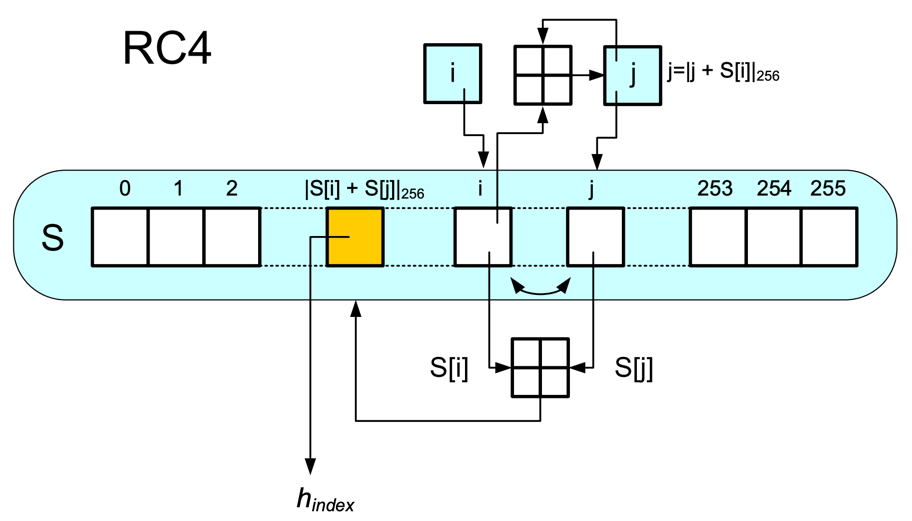
\includegraphics[width=0.5\textwidth]{topics/bi-spol-07/images/rc4}
  \caption{RC4}
\end{figure}

\subsection{Blokové}
\begin{itemize}
\item Bloková šifra je šifrovací systém $(M,C,K,E,D)$, kde $E$ a $D$ jsou zobrazení, definující pro každé $k\in K$ transformaci zašifrování $E_k$ a dešifrování $D_k$ tak, že:
\begin{itemize}
\item zašifrování bloků OT $M=\{m_1,m_2,\dots m_n\}$ probíhá podle vztahu $c_i=E_k(m_i)$ pro každé $i\in N$
\item dešifrování probíhá podle vztahu $m_i = D_k (c_i)$ pro každé $i\in N$.
\end{itemize}
\item Všechny bloky šifrovány stejnou transformací.
\item Zpracováváno po blocích o $t$ znacích abecedy.
\item Blokové šifry využívají principy algoritmů Feistelova typu (použití více zakodování pro posílení šifry).
\item Nejznámější blokové šifry používaly a používají blok o délce 64b: DES, 3DES, \dots
\item V současné době se přechází na blok 128 bitů, který používá standard AES.
\end{itemize}

\subsubsection{DES}
\begin{itemize}
\item Používá 16 rund (iterací) a 64b bloky OT a ŠT.
\item Šifrovací klíč $k$ má délku 56b (protože každý 8 bit je paritní).
\item Po počáteční permutaci je blok rozdělen na dvě 32b poloviny $(L_0,R_0)$. Každá ze 16 rund transformuje $(L_i, R_i)$ na novou hodnotu $(L_{i+1},R_{i+1}) = (R_i, L_i \oplus f(R_i,k_{i+1}))$, liší se jen použitím jiného rundovního klíče $k_i$.
\item Ve funkci probíhají operace expanze, permutace a substituce.
\end{itemize}

\begin{figure}[!ht]
  \centering
  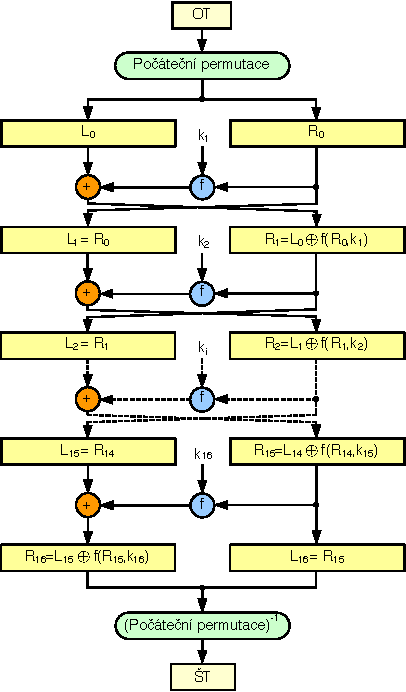
\includegraphics[width=0.3\textwidth]{topics/bi-spol-07/images/des}
  \caption{DES}
\end{figure}

\subsubsection{3DES}
\begin{itemize}
\item 3DES prodlužuje originální DES tím, že používá DES jako stavební prvek celkem 3 krát.
\item Používá dva (112b) nebo tři (168b) různé klíče.
\item Kompatibilní s DES ($k_1=k_2=k_3$).
\item Varianta EDE - Encrypt($k_1$), Decrypt($k_2$), Encrypt($k_3$) -- decrypt je akorát v opačném pořadí a prohodí se E za D (DED).
\end{itemize}

\subsubsection{AES}
\begin{itemize}
\item Náhrada za DES
\item Délka bloku 128 bitů
\item Tři délky klíče: 128, 192 a 256 bitů 
\item Není Feistelova typu
\item SubBytes, ShiftRows, MixColumns, AddRoundKey \dots
\end{itemize}

\section{Operační módy blokových šifer}
Operační módy blokových šifer jsou způsoby použití blokových šifer v daném kryptosystému, kde OT není jen 1 blok blokové šifry, ale obecně posloupnost znaků dané abecedy.

\begin{figure}[ht!]
\centering
\begin{minipage}{.5\textwidth}
  \centering
  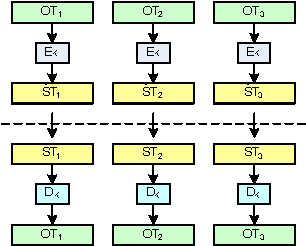
\includegraphics[width=.75\linewidth]{topics/bi-spol-07/images/ecb}
  \caption{ECB - Electronic Code Book}
  \begin{itemize}
    \item Každý blok šifrován zvlášť.
    \item Stejné bloky mají stejný šifrovaný obraz.
    \item Není nijak zaručena integrita, útočník může libovolně měnit bloky.
  \end{itemize}
\end{minipage}%
\begin{minipage}{.5\textwidth}
  \centering
  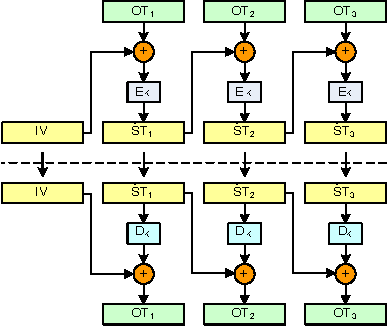
\includegraphics[width=.75\linewidth]{topics/bi-spol-07/images/cbc}
  \caption{CBC - Cipher Block Chaining}
  \begin{itemize}
    \item Nejpoužívanější mód blokových šifer.
    \item Samosynchronizace po 2 blocích.
  \end{itemize}
\end{minipage}
\end{figure}

\begin{figure}[ht!]
\centering
\begin{minipage}{.5\textwidth}
  \centering
  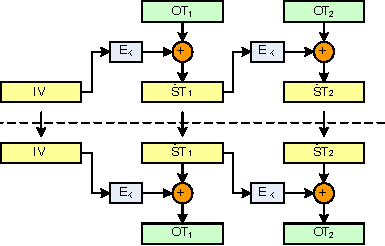
\includegraphics[width=.75\linewidth]{topics/bi-spol-07/images/cfb}
  \caption{CFB - Cipher FeedBack}
  \begin{itemize}
    \item Převádí blokovou šifru na proudovou.
    \item Samosynchronizace po 2 blocích.
    \item Je třeba jenom jedno zobrazení a to šifrovací (to se použije i při dešifrování, jednoduší hw implementace).
  \end{itemize}
\end{minipage}%
\begin{minipage}{.5\textwidth}
  \centering
  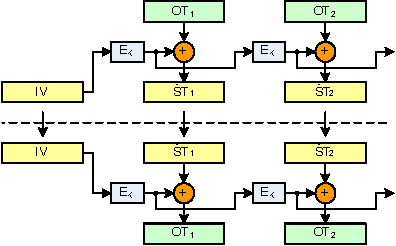
\includegraphics[width=.75\linewidth]{topics/bi-spol-07/images/ofb}
  \caption{OFB - Output FeedBack}
  \begin{itemize}
    \item Převádí blokovou šifru na prodovou.
    \item Synchonní šifra, heslo je generováno zcela nezávisle na OT a ŠT.
    \item Stejně jak CFB stačí pouze šifrování, dešifrování není třeba.
  \end{itemize}
\end{minipage}
\end{figure}

\begin{figure}[ht!]
\centering
\begin{minipage}{.5\textwidth}
  \centering
  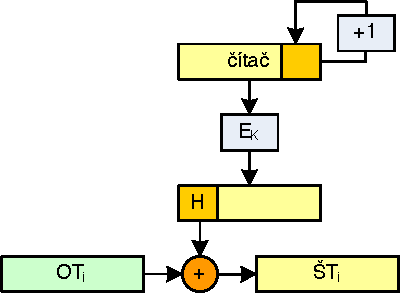
\includegraphics[width=.5\linewidth]{topics/bi-spol-07/images/ctr}
  \caption{CTR - Counter}
  \begin{itemize}
    \item převádí blokovou šifru na asynchronní proudovou šifru.
    \item smyslem je zaručit maximální periodu hesla (pomocí čítače).
    \item výhoda: heslo může být vypočítání jen na základě pozice otevřeného textu a IV, nezávisle na ostaním.
  \end{itemize}
\end{minipage}%
\begin{minipage}{.5\textwidth}
  \centering
  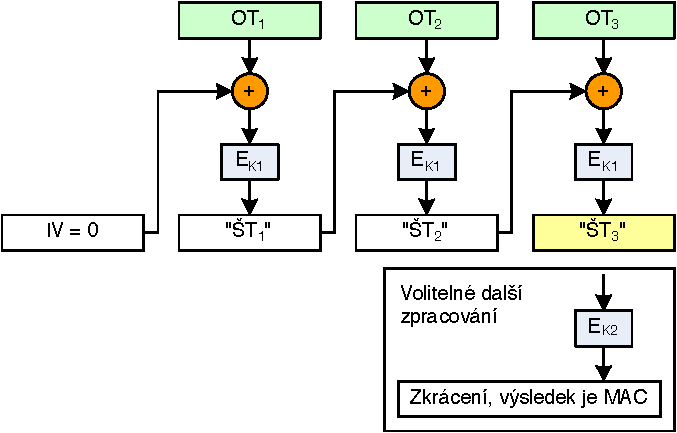
\includegraphics[width=.75\linewidth]{topics/bi-spol-07/images/mac}
  \caption{MAC - Message Authentication Code}
  \begin{itemize}
    \item Řeší neporušitelnost dat.
    \item Podobný jako CBC, ale šifrovaný text se nikam neposílá. 
    \item Použije se jiný utajený klíč.
    \item Nezaručuje nepopíratelnost.
  \end{itemize}
\end{minipage}
\end{figure}


% \begin{definition}
% Nechť množina zpráv M je složená ze všech možných $2n$-tic $V_{2n}$ a prostor klíčů tvoří všechny možné $h$-tice funkci $k=f_1,f_2,\dots,f_h$, $f_i:V_n \to V_n$ pro každé $i=1,2,\dots,h$ a prostor zašifrovaných textů $C=V_{2n}$.
% Zobrazení $T_k:K \times V_{2n}\to V_{2n}$, definované rekurentně vztahy
% \begin{align*}
%   m_{i+1} &= m_{i-1}+f_i(m_i), & \describe{pro $i=1,2,\dots,h$} \\
%   T_k(m)  &= (m_h m_{h+1}),
% \end{align*}
% kde $m=(m_0 m_1)\in M$, definuje \textbf{Feistelův kryptosystém}.
% \end{definition}

\end{document}
